\RequirePackage{luatex85}
\documentclass[border=1mm]{standalone}
\usepackage{myFig}
\begin{document}
\begin{tikzpicture}
  \node (exterior) at (0, 0) {\textbf{外観}};
  \node (interior) at (6.5, 0) {\textbf{論理ICの内部}};
  \node[anchor=south] at (exterior.north) {%
    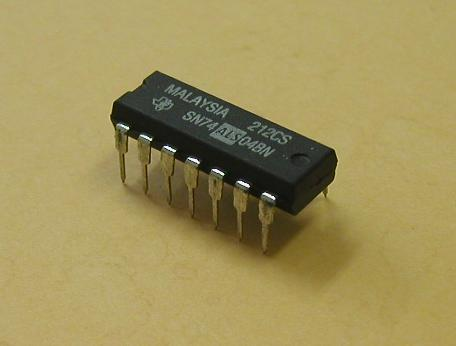
\includegraphics[width=0.45\hsize]{7404.JPG}
  };
  \node[anchor=south] at (interior.north) {
    \begin{tikzpicture}
      \setlength{\tabcolsep}{2pt}
      \node(a){%
	\begin{tabular}{ccl}
	  $V_\mathrm{cc}$&:&5V電源の「$+$」を配線する. \\
	  $\mathrm{GND}$&:&5V電源の「$-$」を配線する.  \\
	\end{tabular}
      };
      \node[anchor=north] (b) at (a.south) {
	\begin{tikzpicture}[circuit logic US]
	  % 枠を置く
	  \draw(0.25, 0) rectangle ++(6.5, 2.5);
	  \draw(0.25, 1) arc (-90:90:0.5cm and 0.25cm);
	  % 端子を配置する
	  \foreach \x [count=\i] in {1,2,...,7}{
	    \node[draw, fill=white, text width=0.3cm,
              align=center, anchor=center](a\x) at (\i*0.9, 0){\small\x};
	  }
	  \foreach \x [count=\i] in {14,13,...,8}{
	    \node[draw, fill=white, text width=0.3cm,
              align=center, anchor=center](a\x)	at (\i*0.9, 2.5){\small\x};
	  }
	  % VccとGNDを置く
	  \node[anchor=south] at (a14.north){$V_\mathrm{cc}$};
	  \node[anchor=north] at (a7.south){$\mathrm{GND}$};
	  % NANDを置く
	  \node[nand gate, anchor=center, 
            scale=0.75] (nand1) at ([yshift=0.75cm]$(a2)!0.5!(a3)$) {};
	  \node[nand gate, anchor=center,
            scale=0.75] (nand2) at ([yshift=0.75cm]$(a5)!0.5!(a6)$) {};
	  \node[nand gate, anchor=center,
            scale=0.75] (nand3) at ([yshift=-0.75cm]$(a12)!0.5!(a11)$) {};
	  \node[nand gate, anchor=center,
            scale=0.75] (nand4) at ([yshift=-0.75cm]$(a9)!0.5!(a8)$) {};
	  \draw(a1) |- (nand1.input 1);
	  \draw(a2) |- (nand1.input 2);
	  \draw(nand1.output) -| (a3);
	  \draw(a4) |- (nand2.input 1);
	  \draw(a5) |- (nand2.input 2);
	  \draw(nand2.output) -| (a6);
	  \draw(a12) |- (nand3.input 1);
	  \draw(a13) |- (nand3.input 2);
	  \draw(nand3.output) -| (a11);
	  \draw(a9)  |- (nand4.input 1);
	  \draw(a10) |- (nand4.input 2);
	  \draw(nand4.output) -| (a8);
	\end{tikzpicture}
      };
    \end{tikzpicture}
  };
\end{tikzpicture}
\end{document}
